\setlength\abovedisplayshortskip{20pt}
\setlength\belowdisplayshortskip{20pt}
\setlength\abovedisplayskip{20pt}
\setlength\belowdisplayskip{20pt}





\section{Auswertung}

Die aus dem Versuch S1 erhaltenen Daten wurden in Abbildung \ref{HCLplot} für HCl und in Abbildung \ref{COplot} für CO graphisch dargestellt. Der mittels Igor Pro ausgegebene Fit, sowie die dadurch erhaltenen Koeffizienten der Morsefunktion sind ebenfalls in den Abbildungen zu erkennen.
%%%%%%%%%%%%%%%%%%%%%%%%%%
\begin{figure}[H]
	\centering	
	\begin{minipage}{1\textwidth}
	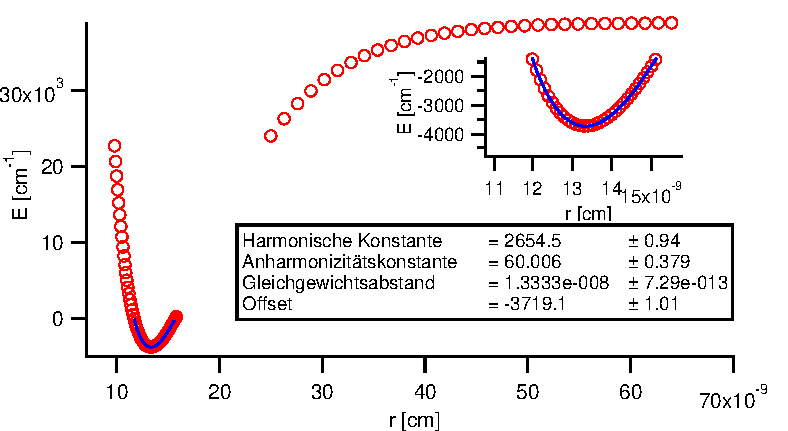
\includegraphics[width=\columnwidth]{Bilder/HCLGraph.pdf}
	\end{minipage}
	
	
	\caption{mit IgorPro gemacht. HCL über morsefit}
	

	\label{HCLplot}
\end{figure}
%%%%%%%%%%%%%%%%%%%%%%%%%%%	
\begin{figure}[H]
	\centering	
	\begin{minipage}{1\textwidth}
	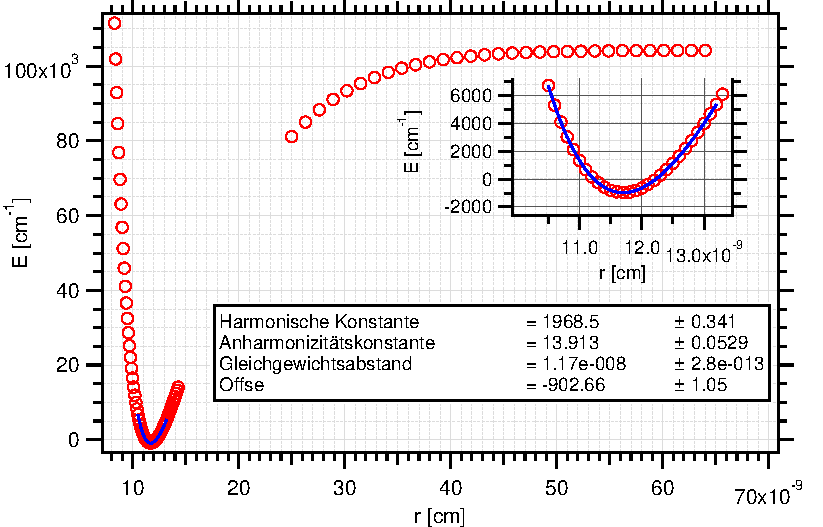
\includegraphics[width=\columnwidth]{Bilder/Graph2.pdf}
	\end{minipage}
	
	
	\caption{mit IgorPro gemacht. CO über morsefit}
	
	
	\label{COplot}
\end{figure}
%%%%%%%%%%%%%%%%%%%%%%%






Mittels den erhaltenen Koeffizienten war es nun möglich die theorethische Dissoziationsenergie, sowie die Rotationskonstante B zu berechnen. Die berechneten Werte wurden neben den aus dem Fit erhaltenen Koeffizienten in Tabelle \ref{tab:zusammen} zusammengetragen und den Literaturdaten im Vergleich gegenübergestellt.


 \begin{table}[H]

 
 
 \caption{Für CO und HCl erhaltene Koeffizienten aus dem Fit der Morsefunktion sowie die berechneten Rotationskonstanten und Dissoziationsenergien.}
\begin{tabular}{L{0.1\linewidth}L{0.1\linewidth}L{0.2\linewidth}L{0.2\linewidth}L{0.25\linewidth}}

 
  Molekül  &  &  Wert &   Absoluter Fehler & Literatur \\
  \addlinespace[1ex]
\hline
\addlinespace[1ex]
  CO  & $\tilde{\nu}_e$ &\SI[mode=math]{1968.5}{cm^{-1}} &\SI[mode=math]{0.35}{cm^{-1}} &\SI[mode=math]{2169}{cm^{-1}} \\
  CO  & $\tilde{\nu}_e x_e$& \SI[mode=math]{13.91}{cm^{-1}}&\SI[mode=math]{0.05}{cm^{-1}}&\SI[mode=math]{13.28831}{cm^{-1}} \\
  CO  & $r_e$&\SI[mode=math]{11.7000e-9}{cm} & \SI[mode=math]{0.0003e-9}{cm}&\SI[mode=math]{11.28323e-9}{cm}\\
  CO  & $D_e$&\SI[mode=math]{}{}&\SI[mode=math]{}{}\\
    CO&$B$&	\SI[mode=math]{2}{cm^{-1}}&\SI[mode=math]{1}{cm^{-1}}&\SI[mode=math]{1.93128087}{cm^{-1}}\\
\addlinespace[1ex]
\hline
\addlinespace[1ex]
  HCl  & $\tilde{\nu}_e$ &\SI[mode=math]{2654}{cm^{-1}} &\SI[mode=math]{1}{cm^{-1}} &\SI[mode=math]{2990.946}{cm^{-1}} \\
  HCl  & $\tilde{\nu}_e x_e$& \SI[mode=math]{60.0}{cm^{-1}}&\SI[mode=math]{0.5}{cm^{-1}}&\SI[mode=math]{52.8186}{cm^{-1}} \\
  HCl  & $r_e$&\SI[mode=math]{13.3333e-9}{cm} & \SI[mode=math]{0.0008e-9}{cm}&\SI[mode=math]{12.7455e-8}{cm}\\
  HCl  & $D_e$&\SI[mode=math]{}{}&\SI[mode=math]{}{}\\
    HCl&$B$&	\SI[mode=math]{13.00}{cm^{-1}}&\SI[mode=math]{0.07}{cm^{-1}}&\SI[mode=math]{10.59341}{cm^{-1}}\\
\addlinespace[1ex]
\hline   
   
 \end{tabular}
 \label{tab:zusammen}
 \end{table}














\subsection{Berechnung der Dissoziationsenergie}
Die Dissoziationsenergie ermittelt sich gemäß Gleichung \ref{eq:de}
\begin{equation} 
	\label{eq:de}
		D_e \approx \frac{\tilde{\nu}_e^2}{4 \tilde{\nu}_e x_e}
\end{equation}

%%%%%%%%%%%%%%%%%%%%%%
Der absolute Fehler berechnet sich nach Gleichung \ref{eq:Deltade}.
\begin{equation} 
	\label{eq:Deltade}
		\Delta D_e =\left|\frac{\delta D_e}{\delta \tilde{\nu}_e}\right|\cdot \Delta \tilde{\nu}_e + \left|\frac{\delta D_e}{\delta \tilde{\nu}_e x_e}\right|\cdot \Delta \tilde{\nu}_e x_e 
\end{equation}
Somit gilt für die Dissoziationsenergie für CO nach Gleichung \ref{eq:Rede}.
\begin{equation} 
	\label{eq:Rede}
		D_e \approx \frac{2654.5^2}{4\cdot60.006} ~\si
{cm^{-1}}  \approx  \SI[mode=math]{29356.94}{cm^{-1}} 
\end{equation}
sowie deren absoluten Fehler nach Gleichung 

%%%%%%%%%%%%%%
%\begin{itemize}
% \item \FPeval{\result}{clip((2654.5^2)/(60.006*4))}%
%    $\result$
%\end{itemize} 








\subsection{Berechnung der Rotationskonstante B}
\subsubsection*{Allgemeines Vorgehen}
Die Rotationskonstante $B$, sowie der Fehler $\Delta B$ berechnen sich gemäß der Gleichungen \ref{eq:B} und \ref{eq:DeltaB}.
\begin{align}
B 	
   			&= \frac{\hbar}{4 \cdot \pi \cdot c \cdot \mu  \cdot r_e^{2}}
   			\notag\\\label{eq:B}
   			&= konst.\cdot\frac{1}{\mu  \cdot r_e^{2}}
   			\\\label{eq:DeltaB}	
\Delta B	
   			&=  \left|\frac{\delta B}{\delta r_e}\right|\cdot\Delta r_e =konst. \cdot\left|\frac{-2}{\mu \cdot r_e^{3}  }\right|\cdot \Delta r_e  	
   			\end{align}
Dabei werden zur Vereinfachung die Naturkonstante in einer Konstante $konst.$ in Gleichung \ref{eq:konst} zusammengefasst.


\begin{align}
\label{eq:konst}
konst.&= 			 \frac{\SI[mode=math]{1.054571800e-34}{kg.m.s^{-1}}}{4\cdot 3.14159265359 \cdot \SI[mode=math]{299792458}{m.s^{-1}}}=\SI[mode=math]{2.799274682e-44}{kg.m}  				
\end{align}






\subsubsection*{Berechnung für HCl}
Für HCl ergibt sich somit, unter Verwendung der durch den Fit ausgegeben Gleichgewichtsabstand $r_e$ und dem dazugehörigen absoluten Fehler $\Delta r_e$
\begin{align}
\label{eq:re_HCL}
r_e &= 1.3333 \cdot 10^{-8} ~\si{cm}=\SI[mode=math]{1.3333e-10}{m}
\\
\Delta r_e &= 7.29 \cdot 10^{-13} ~\si{cm}=\SI[mode=math]{7.29e-13}{m}
\end{align}
,sowie der in Gleichung \ref{eq:mu_HCL} berechneten reduzierten Masse $\mu$
\begin{align}
\mu&= \frac{m(H)\cdot m(Cl)}{m(H)+m(Cl)}\notag\\
\mu&= \frac{1\cdot35}{1+35} ~\si{u}=\frac{35}{36}~\si{u}=\SI[mode=math]{1.614412705e-27}{kg}\label{eq:mu_HCL}
\end{align}
die in Gleichung \ref{eq:B_HCL} berechnete Rotationskonstante $B$
\begin{align}
\label{eq:B_HCL}
B &=\frac{\SI[mode=math]{2.799274682e-44}{kg.m}}{\SI[mode=math]{1.614412705e-27}{kg}\cdot\SI[mode=math]{1.3333e-20}{m^{2}}}
&=\SI[mode=math]{1300.478182}{m^{-1}}
=\SI[mode=math]{13}{cm^{-1}}
\end{align}


,sowie der absolute Fehler $\Delta B$  gemäß Gleichung  \ref{eq:DeltaB_HCL}.  
\begin{align}
\Delta B &= \left|-2\cdot \frac{\SI[mode=math]{2.799274682e-44}{kg.m}}{\SI[mode=math]{1.614412705e-27}{kg}\cdot\SI[mode=math]{1.3333e-30}{m^{3}}}\right| \cdot \SI[mode=math]{7.29e-15}{m}
\notag\\
&=  \SI[mode=math]{0.07282667818}{m}= \SI[mode=math]{7.5}{cm} \label{eq:DeltaB_HCL}
\end{align} 






\subsubsection*{Berechnung für CO}
Für CO ergibt sich somit, unter Verwendung der durch den Fit ausgegeben Gleichgewichtsabstand $r_e$ und dem dazugehörigen absoluten Fehler $\Delta r_e$
\begin{align}
\label{eq:r_CO}
r_e &= 1.17 \cdot 10^{-8} ~\si{cm}=\SI[mode=math]{1.17e-10}{m}
\\
\Delta r_e &= 2.8 \cdot 10^{-13} ~\si{cm}=\SI[mode=math]{2.8e-15}{m}
\end{align}
 sowie der in Gleichung \ref{eq:mu_CO} berechneten reduzierten Masse $\mu$
\begin{align}
\mu&= \frac{m(H)\cdot m(Cl)}{m(H)+m(Cl)}\notag\\
\mu&= \frac{12\cdot16}{12+16} ~\si{u}=\frac{48}{7}~\si{u}=\SI[mode=math]{1.138655165e-26}{kg}\label{eq:mu_CO}
\end{align}
die in Gleichung \ref{eq:B_CO} berechnete Rotationskonstante $B$
\begin{align}
\label{eq:B_CO}
B &=\frac{\SI[mode=math]{2.799274682e-44}{kg.m}}{\SI[mode=math]{1.13655165e-26}{kg}\cdot\SI[mode=math]{1.17e-20}{m^{2}}}
&=\SI[mode=math]{210.50}{m^{-1}}
=\SI[mode=math]{2}{cm^{-1}}
\end{align}


,sowie der absolute Fehler $\Delta B$ gemäß der  Gleichung \ref{eq:DeltaB_CO}.  
\begin{align}
\Delta B &= \left|-2\cdot \frac{\SI[mode=math]{2.799274682e-44}{kg.m}}{\SI[mode=math]{1.13655165e-26}{kg}\cdot\SI[mode=math]{1.17e-30}{m^{3}}}\right| \cdot \SI[mode=math]{2.8e-15}{m}
\notag\\
&=\SI[mode=math]{0.01178849883 }{m} = \SI[mode=math]{1}{cm}   \label{eq:DeltaB_CO}
\end{align} 









 %ab hier die Fehlerrechnung  
 
%&eingesetzt in die Gleichung \ref{eq:de} ergibt sich somit:
%hier eine Abblidung\\[5ex]
%Anpassung der Parameter an die Morsefunktion\\[5ex]
%Rechnerische Bestimmung der molekularen Konstanten 
%aus der Morsefunktoin\\[5ex]
%Tabelarische Auflistung für CO und HCl + Literaturdaten\\[5ex]
%Prognose des Rotationsschwingungsspektrum von HF und HCl.




\subsection{Roationsschwingungsspektren bei verschiedenen Temperaturen}
\subsection*{CO}

Die erhaltene Rotationskonstante $B$ sowie $\tilde{\nu}_e$ und $\tilde{\nu}_e x_e$ wurden verwendet um das theoretische Aussehen der Rotationsschwingungsspektren von HCl und CO bei \SI[mode=math]{1000}{K}, \SI[mode=math]{100}{K}, \SI[mode=math]{10}{K}, \SI[mode=math]{1}{K} und \SI[mode=math]{0.01}{K} vorherzusagen.

\begin{figure}[H]
\centering	
	\begin{minipage}{0.8\linewidth}
	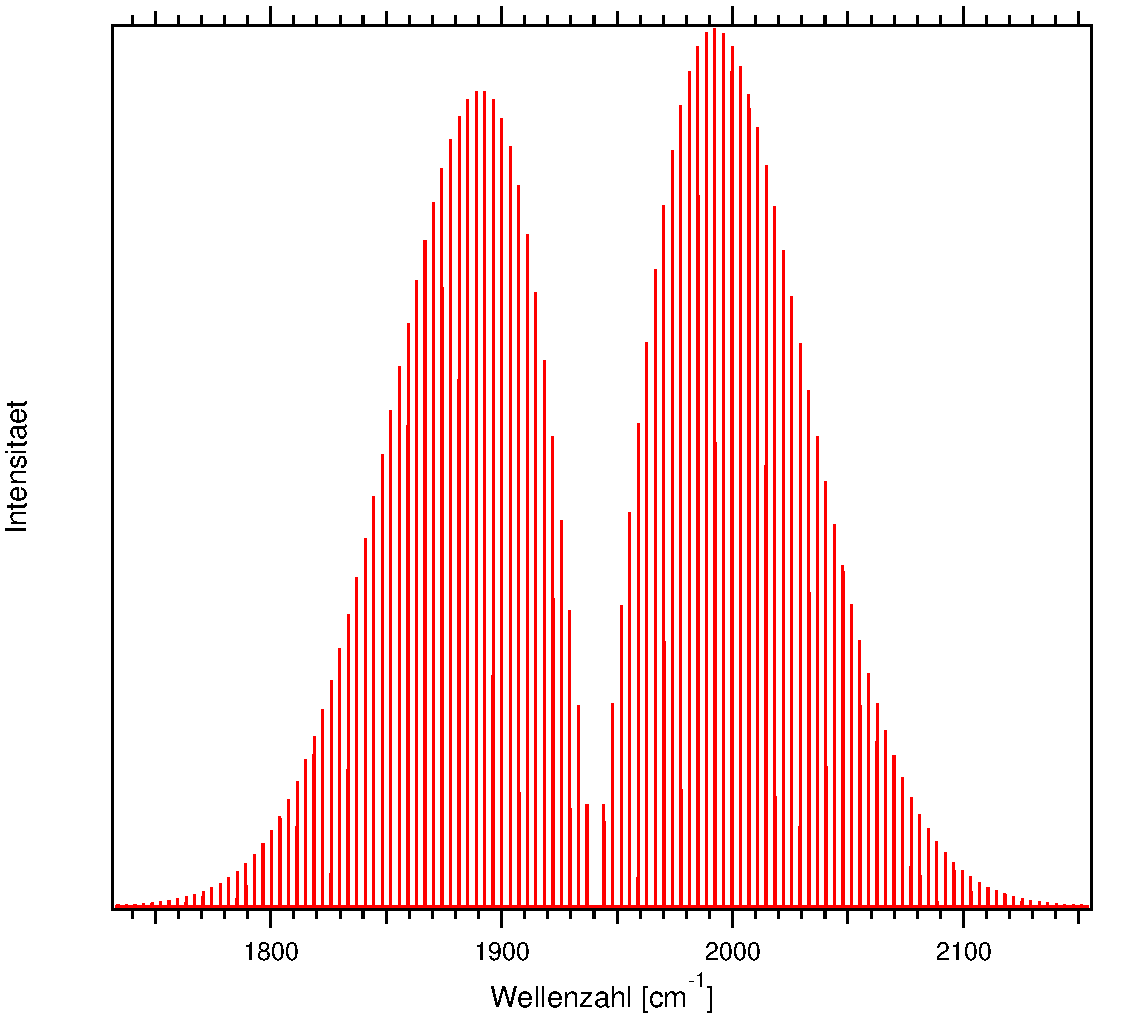
\includegraphics[width=\linewidth]{Bilder/1000CO.pdf}
	\caption{berechnetes Rotationsschwingungsspektrum bei 10~K}
	\end{minipage}

	
	
	
	\label{Rot:1000CO}
\end{figure}

\begin{figure}[H]
	
	\begin{minipage}{0.5\textwidth}
	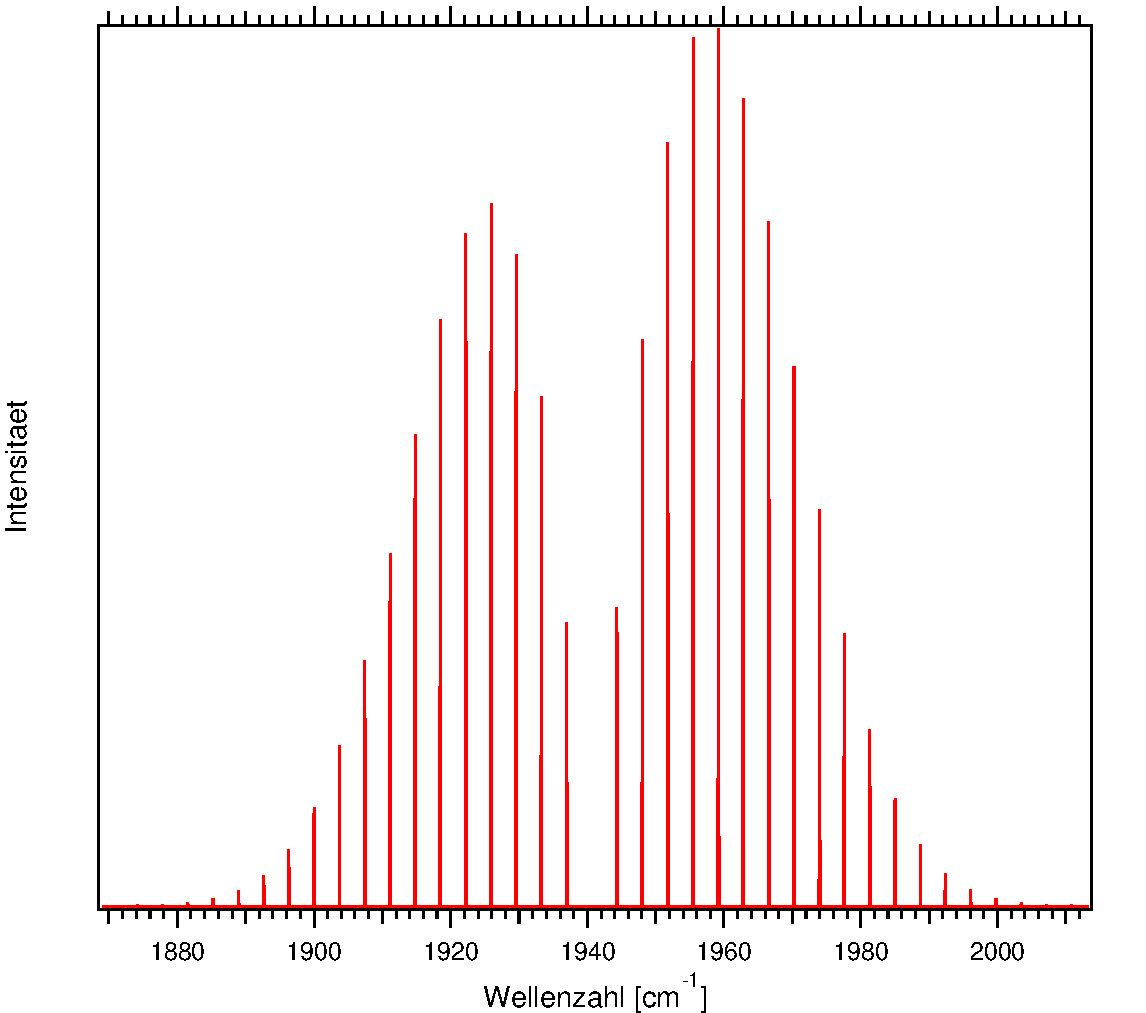
\includegraphics[width=\textwidth]{Bilder/100CO.pdf}
	\caption{berechnetes Rotationsschwingungsspektrum bei 1000 Kelvin}
	\end{minipage}
\begin{minipage}{0.5\textwidth}
	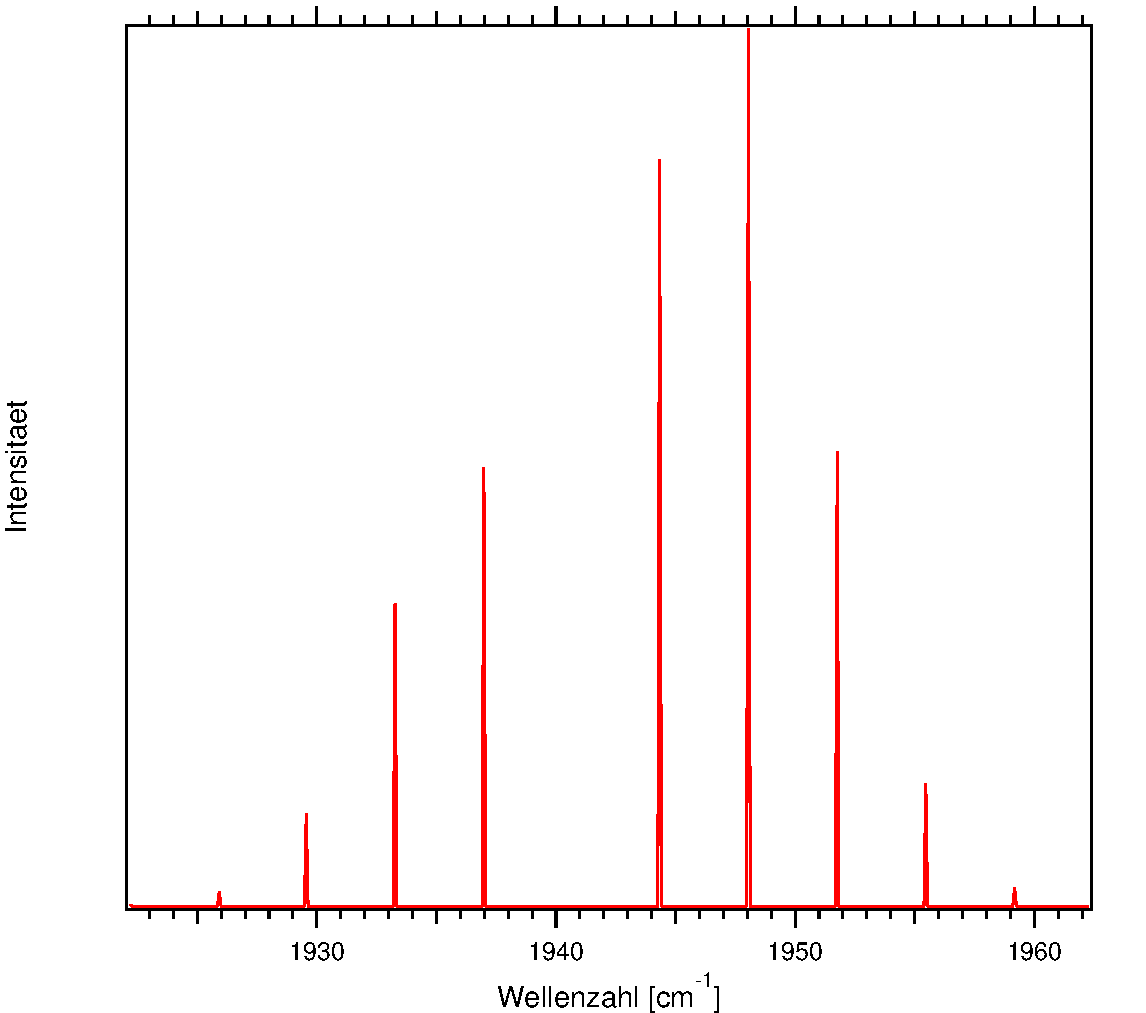
\includegraphics[width=\textwidth]{Bilder/10CO.pdf}
	\caption{berechnetes Rotationsschwingungsspektrum bei 100 Kelvin}
	\end{minipage}	
	
		
	\label{Rot:10CO}
\end{figure}

\begin{figure}[H]
\centering	
	\begin{minipage}{0.47\linewidth}
	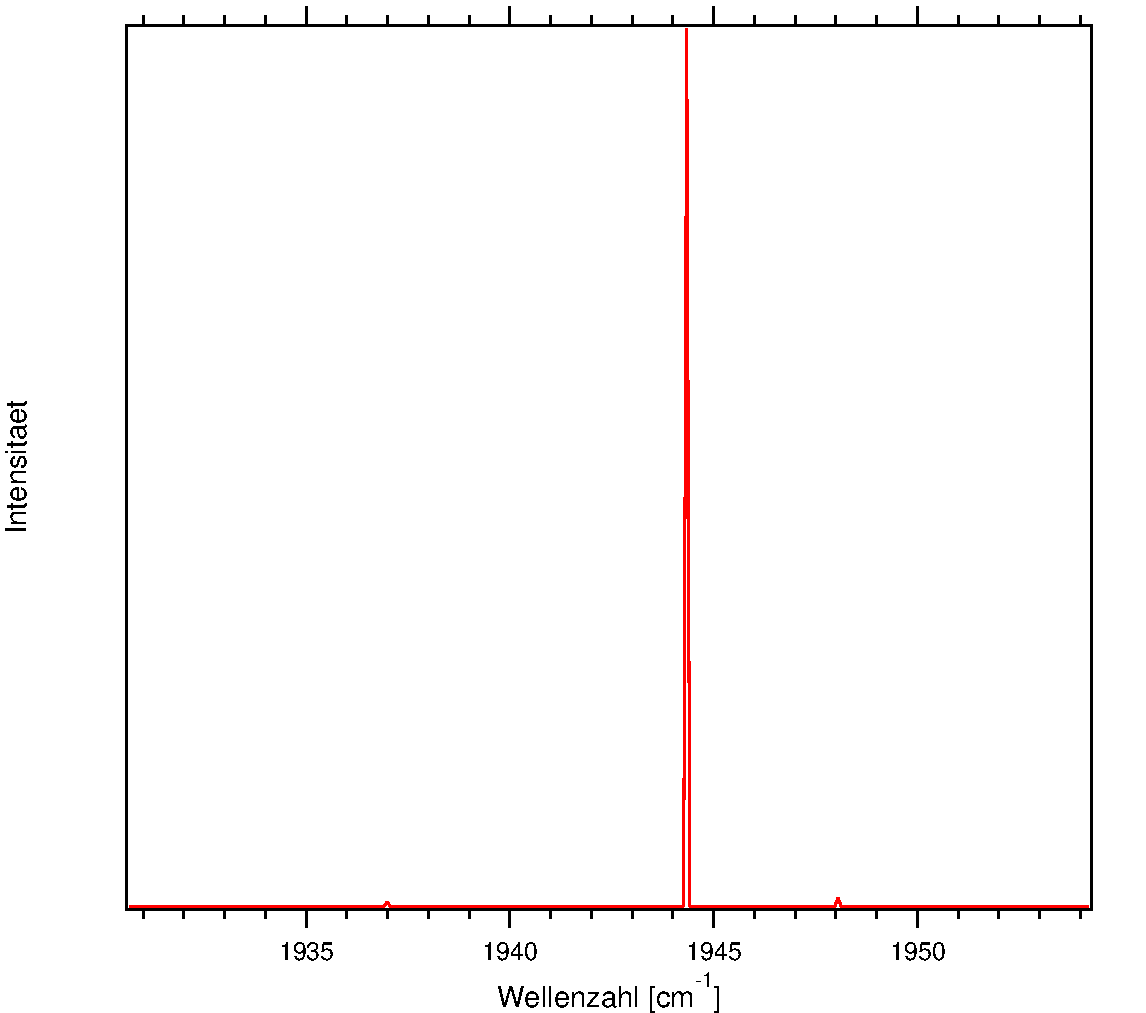
\includegraphics[width=\linewidth]{Bilder/1CO.pdf}
	\caption{berechnetes Rotationsschwingungsspektrum bei 10~K}
	\end{minipage}
\begin{minipage}{0.47\linewidth}
	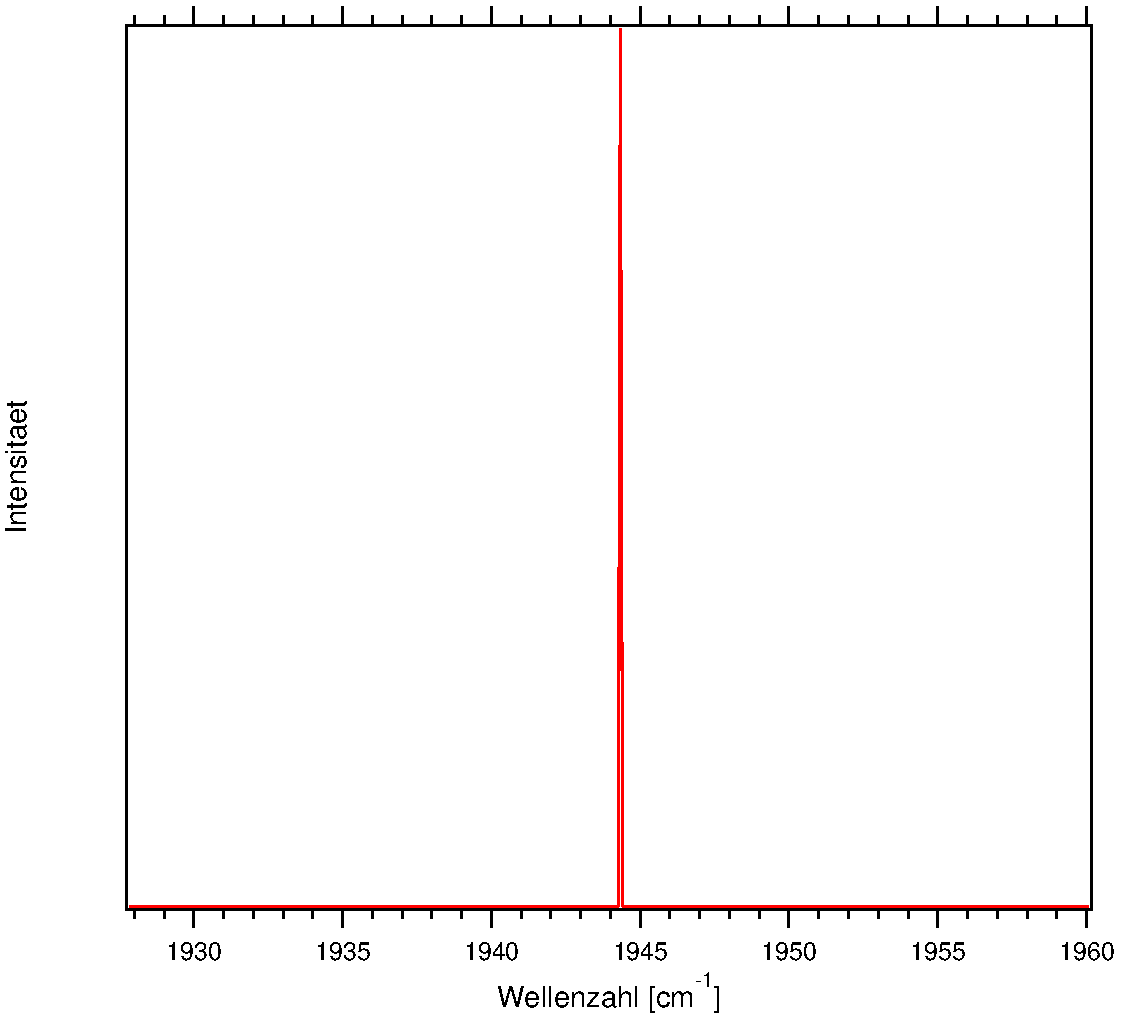
\includegraphics[width=\linewidth]{Bilder/001CO.pdf}
	\caption{berechnetes Rotationsschwingungsspektrum bei 1~K}
	\end{minipage}
	
	
	
	
	\label{Rot:001CO}
\end{figure}





\subsection*{HCl}

\begin{figure}[H]
	
	\begin{minipage}{0.5\textwidth}
	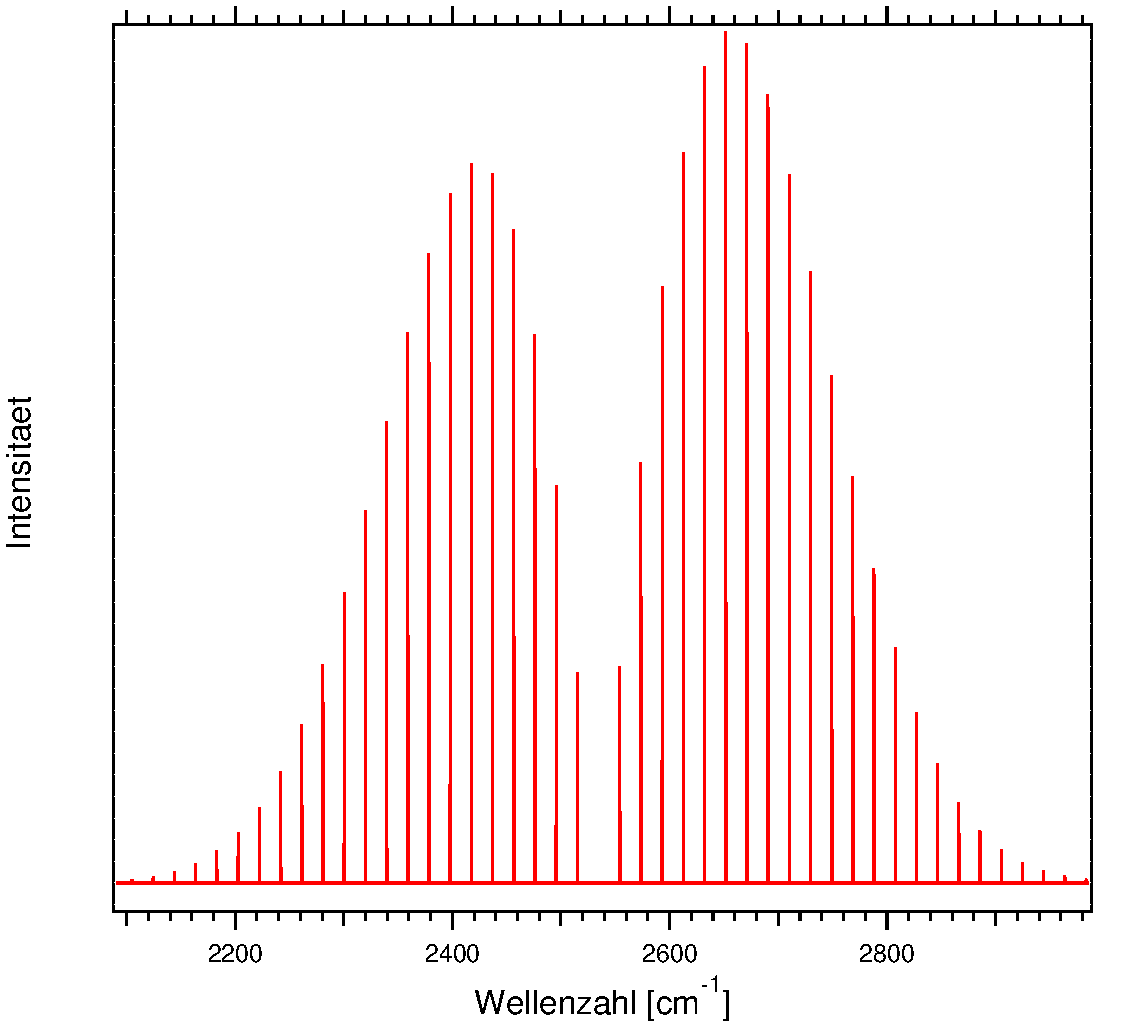
\includegraphics[width=\textwidth]{Bilder/1000HCL.pdf}
	\caption{berechnetes Rotationsschwingungsspektrum bei 1000 Kelvin}
	\end{minipage}
\begin{minipage}{0.5\textwidth}
	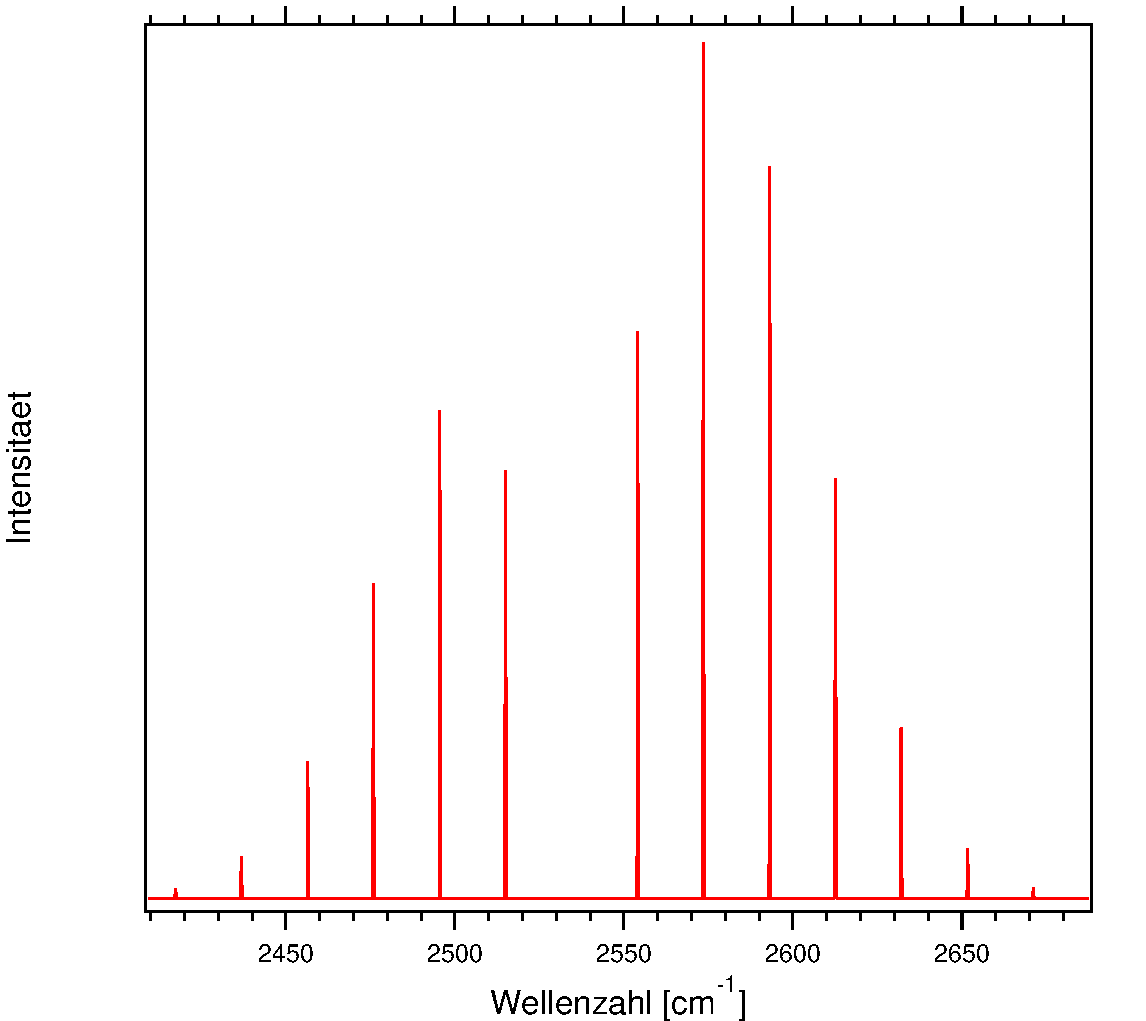
\includegraphics[width=\textwidth]{Bilder/100HCL.pdf}
	\caption{berechnetes Rotationsschwingungsspektrum bei 100 Kelvin}
	\end{minipage}	
	
	\caption{HCL 1000 und 100 Kelvin}
	
	
%	\label{1}
\end{figure}

\begin{figure}[H]
\centering	
	\begin{minipage}{0.47\linewidth}
	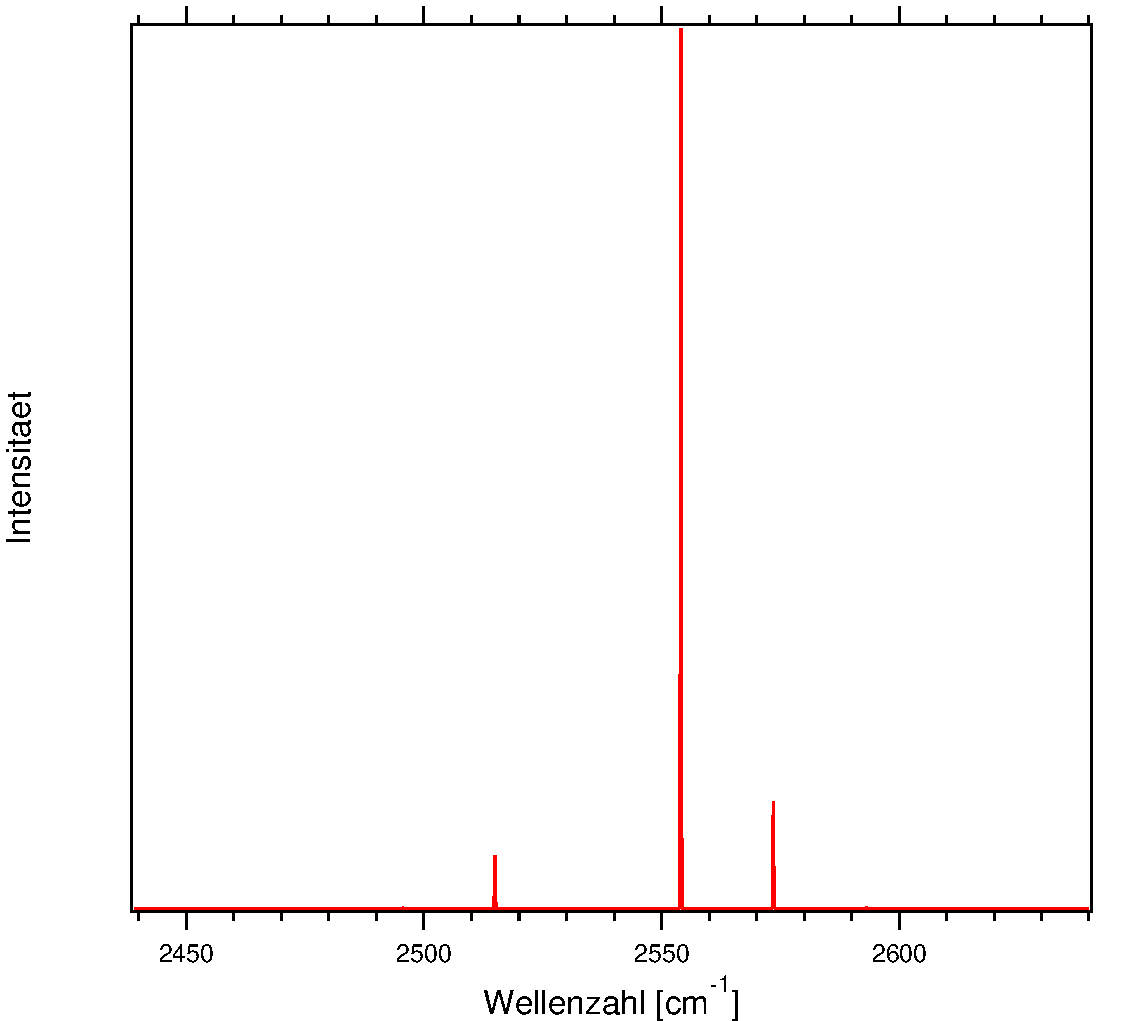
\includegraphics[width=\linewidth]{Bilder/10HCL.pdf}
	\caption{berechnetes Rotationsschwingungsspektrum bei 10~K}
	\end{minipage}
\begin{minipage}{0.47\linewidth}
	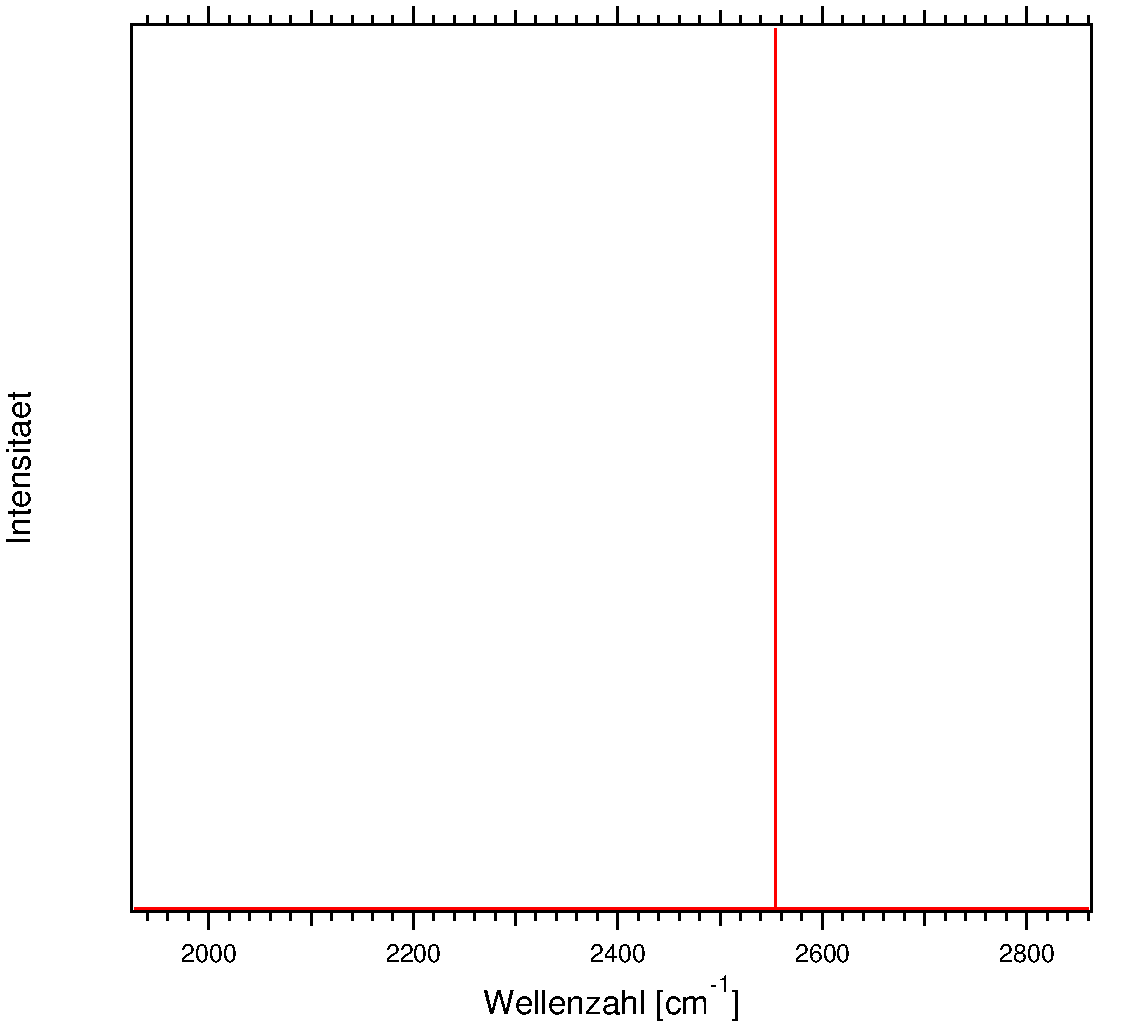
\includegraphics[width=\linewidth]{Bilder/1HCL.pdf}
	\caption{berechnetes Rotationsschwingungsspektrum bei 1~K}
	\end{minipage}
	
	\caption{HCL 10 und 1 Kelvin}
	
	
	
\end{figure}

\begin{figure}[H]
\centering	
	\begin{minipage}{0.47\linewidth}
	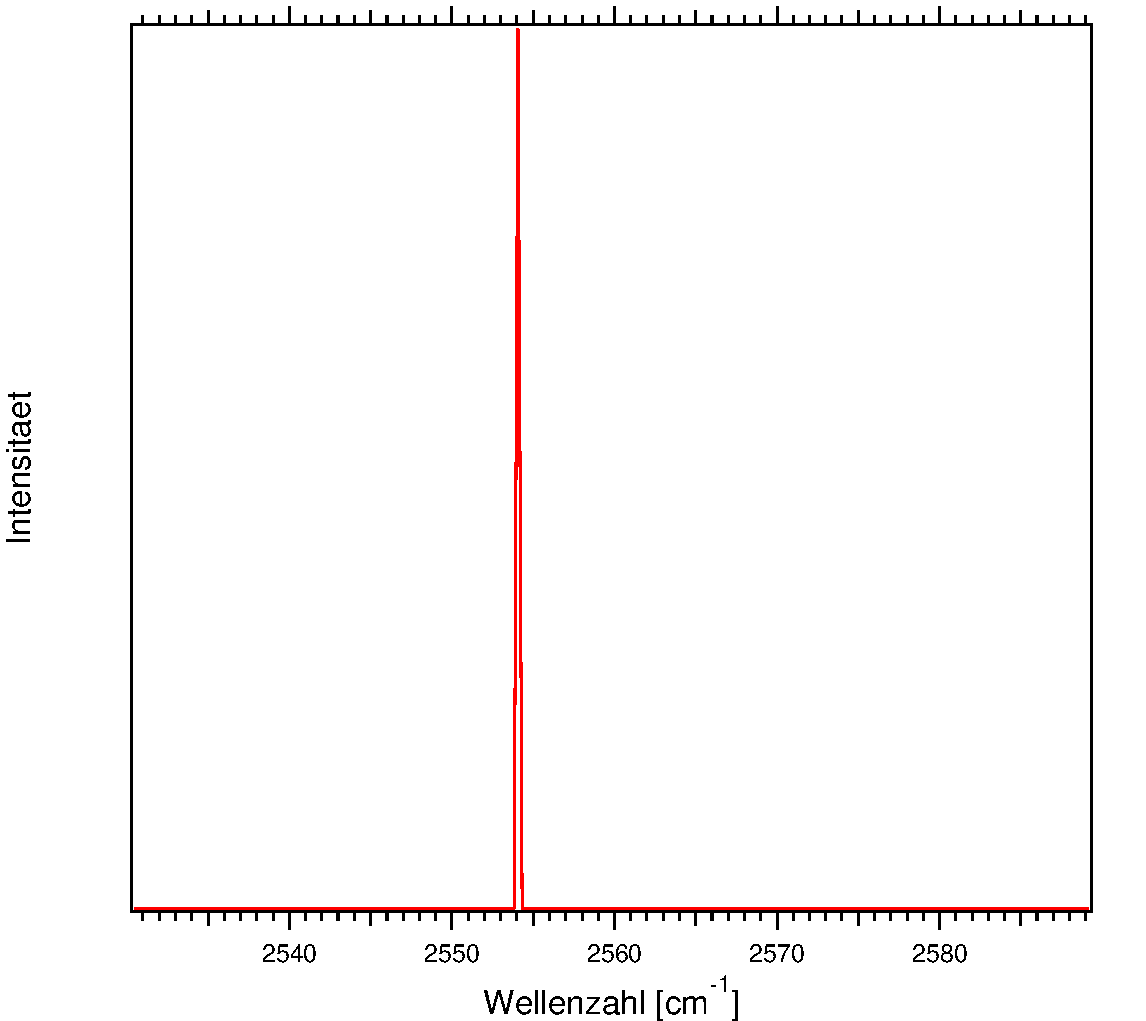
\includegraphics[width=\linewidth]{Bilder/001HCL.pdf}
	\caption{berechnetes Rotationsschwingungsspektrum bei 10~K}
	\end{minipage}

	\caption{HCL 10 und 1 Kelvin}
	
	
%	\label{3}
\end{figure}

Bilden Sie daraus einen Satz Abbildungen und erklären Sie die Beobachtung! Wieviel Linien erhält man für T=0.01K? Zu welchem Zweig gehört sie? (-1 geht nicht daher +1)
\section{Rohdaten}

